\documentclass[aps,twocolumn,amsmath,amssymb,showpacs,prb,
superscriptaddress,unsortedaddress]{revtex4}
\usepackage{epsf}
\usepackage{graphicx}

\newcommand{\etal}{{\it et al.}}

\begin{document}

\title{Controlling the carrier concentration of the high temperature
superconductor Bi$_2$Sr$_2$CaCu$_2$O$_{8+\delta}$ in Angle Resolved
Photoemission Spectroscopy (ARPES) experiments}

\author{A. D. Palczewski}
\affiliation{Ames Laboratory and Department of Physics and Astronomy,
Iowa State University, Ames, IA 50011, USA}

\author{T. Kondo}
\affiliation{Ames Laboratory and Department of Physics and Astronomy,
Iowa State University, Ames, IA 50011, USA}

\author{J. S. Wen}
\affiliation{Condensed Matter Physics and Materials Science
Department, Brookhaven National Laboratory, Upton, New York 11973, USA
}

\author{G. Z. J. Xu}
\affiliation{Condensed Matter Physics and Materials Science
Department, Brookhaven National Laboratory, Upton, New York 11973, USA
}

\author{G. Gu}
\affiliation{Condensed Matter Physics and Materials Science
Department, Brookhaven National Laboratory, Upton, New York 11973, USA
}

\author{A. Kaminski}
\affiliation{Ames Laboratory and Department of Physics and Astronomy,
Iowa State University, Ames, IA 50011, USA}


\date{\today}

\begin{abstract}
We study the variation of the electronic properties at the surface of
a high temperature superconductor as a function of vacuum conditions
in angle resolved photoemission spectroscopy (ARPES) experiments.
Normally, under less than ideal vacuum conditions the carrier
concentration of Bi$_2$Sr$_2$CaCu$_2$O$_{8+\delta}$ (Bi2212) increases
with time due to the absorption of oxygen from CO$_2$  and CO
molecules that are prime contaminants present in ultra high vacuum
(UHV) systems. We find that in a high quality vacuum environment at
low temperatures, the surface of Bi2212 is quite stable (the carrier
concentration remains constant), however at elevated temperatures the
carrier concentration decreases due to the loss of oxygen atoms from
the Bi-O layer. These two effects can be used to control the carrier
concentration \textit{in-situ}. Our finding opens the possibility of
studying the electronic properties of the cuprates as a function of
doping across the phase diagram on the \textit{same} piece of sample
(i.e. with the same impurities and defects). We envision that this
method could be utilized in other surface sensitive techniques such as
scanning tunneling microscopy/spectroscopy.
\end{abstract}


\pacs{74.70.Dd, 71.18.+y, 71.20.-b, 71.27.+a}

\maketitle

\section{Introduction}

Surface techniques have played an important role in understanding the
properties of the high temperature superconductors. They have revealed
a number of fascinating phenomena such as the direct observation of
the superconducting gap\cite{OLSON} and its
anisotropy\cite{SHENSC,HONGSC}, confirmation of the d-wave symmetry of
the order parameter, direct observation of the pseudogap and its
anisotropy\cite{HONGPG, LOESERPG,MIKEPG}, discovery of spatial
inhomogeneities\cite{DAVIS,YAZDANI},unusual spatial
ordering,\cite{DAVISCHECKER} nodal quasiparticles\cite{KAMINSKIQP},
renormalization effects\cite{VALLA,BOGDANOV,KAMINSKIKINK} and many
others\cite{SHENREVIEW,JCREVIEW}. The success of these techniques rely
on the fact that the layers in some cuprates are very weakly bonded
via the Van der Waals interaction. In such cases the bulk properties
and surface properties are essentially identical, since there is no
charge exchange between the layers. The samples in such cases can be
thought of as a stack of very weakly electrically coupled
2-dimensional conducting surfaces rather than a 3-dimentional object.
Two of the most commonly studied materials with this property are
Bi$_2$Sr$_2$CaCu$_2$O$_{8+\delta}$ (Bi2212) and
Bi$_2$Sr$_2$CuO$_{6+\delta}$ (Bi2201). There is however one important
aspect that needs to be carefully considered, namely the stability of
the cleaved samples under ultra high vacuum (UHV) conditions. UHV is a
rather broad term and refers to pressures lower than
1$\times$10$^{-9}$ Torr. Quite often such conditions are not
sufficient to guarantee the stability of the surface, particularly in
the case of non-stoichiometric materials such as the cuprates. These
problems were recognized early on\cite{SHEN1}, and subsequent
measurements revealed significant changes in the electronic properties
as a function of time after cleaving. This issue was not carefully
examined following these first measurements, and it is likely an
important source of data discrepancies among the various groups
\cite{SHENREVIEW,JCREVIEW}.

Here we present a systematic study of the electronic properties of
Bi2212 as a function of vacuum conditions.  We demonstrate that under
poor vacuum conditions increased carrier concentration arises due to
the breakup of CO and CO$_2$ molecules by exposure to vacuum
ultra-violet (VUV) photons and the subsequent adsorption of oxygen
into the BiO layers. We show that with a UHV leak a sample can
increase it carrier concentration just by sitting in the vaccum.  This
observation confirms that bilayer splitting is only observed in
over-doped Bi2212.  When the partial pressure of active gases is kept
at low levels, the lifetime of cleaved surface of Bi2212 can be as
long as a few weeks at low temperatures (T$<$150K). At elevated
temperatures (T$>$200K) the sample surface loses oxygen, which results
in the reduction of carrier concentration. This second effect is most
likely responsible for the recently reported non-monotonic temperature
dependence of the pseudogap\cite{A. A. Kordyuk 2008}, where at
elevated temperatures the sample surface becomes underdoped and
therefore develops a pseudogap. We demonstrate that these two effects
(\textit{in-situ} absorption and desorption of oxygen) can be utilized
to control the carrier concentration of the sample surface. This
approach enables one to study the intrinsic electronic properties
(i.e. without changing the impurities and defects) of the cuprates
across the phase diagram.

\section{Experimental Details}

The ARPES data was acquired using a laboratory-based Scienta 2002
electron analyzer and high intensity Gammadata UV4050 UV source  with
custom designed optics. The photocurrent at the sample was
approximately 1 $\mu A$, which corresponds to roughly 10$^{13}$
photons/sec at 0.05\% of the bandwidth. The energy resolution was set
at 10 meV and momentum resolution at 0.12$^{\circ}$ and 0.5$^{\circ}$
along a direction parallel and perpendicular to the analyzer slits,
respectively. Samples were mounted on a variable temperature cryostat
(10-300K) cooled by a closed cycle refrigerator. The precision of the
sample positioning stage was 1$\mu m$. The partial pressure of the
active gases was at the detection limit of the Residual Gas Analyzer
(RGA) and the pressure of hydrogen was below 3$\times$10$^{-11}$ Torr.
Excellent vacuum conditions were achieved by strict adherence to good
vacuum practices, use of UHV compatible materials and a cumulative
bake-out time of the system in excess of 6 months. The typical
lifetime of the optimally doped Bi2212 surfaces was greater than two
weeks after cleaving, defined as less than 5\% change of the
superconducting gap (2 meV) at 40K.  The core-level spectra was
acquired on the Hermon beam-line at the Synchrotron Radiation Center
using a Scienta 2002 end-station. The photon energy was set at 500 eV
and energy resolution at 200 meV.


\section{Increasing carrier concentration}

It has been known for some time that aging (increased surface doping)
in the cuprates is caused by less than ideal UHV
conditions\cite{SHEN1}.  Aging is usually detected by measuring the
superconducting gap (the energy gap as defined by the difference
between the peak position of a Bi2212 spectrum and the chemical
potential measured by a polycrystalline gold sample) as a function of
time.  If the gap shifts to a lower binding energy the sample has
aged.\cite{H. Ding 1997,P. Schwaller 2000}.  Fig. 1 (a)-(b) shows an
example of this where a freshly cleaved Bi2212 single crystal was
scanned in a relatively poor vacuum to see how the spectrum changed
over time. A shift to lower binding energy as well as a peak
suppression was detected showing the sample was aging.  In Fig. 1 (c)
the size of the superconducting gap is shown as a function of time.
Only when there were VUV photons on the sample did the sample age.
While there we no VUV photons on the sample, from 5 hour to 21 hours,
the aging stopped. If the non-VUV scanning time is taken out Fig. 1
(d), the magnitude of the gap shows an exponential decay (blue line).
While it is know that surface aging of Bi2212 happens in a poor UHV
system, only when there were VUV photons on the sample does did sample
actually age, signaling that aging is directly related to having VUV
photons on the sample, not just the vacuum conditions. 
%%%%%%%%%%%%%%%%%%%%% aging over time with break and without, carbon
core levels and select cuts
\begin{figure}
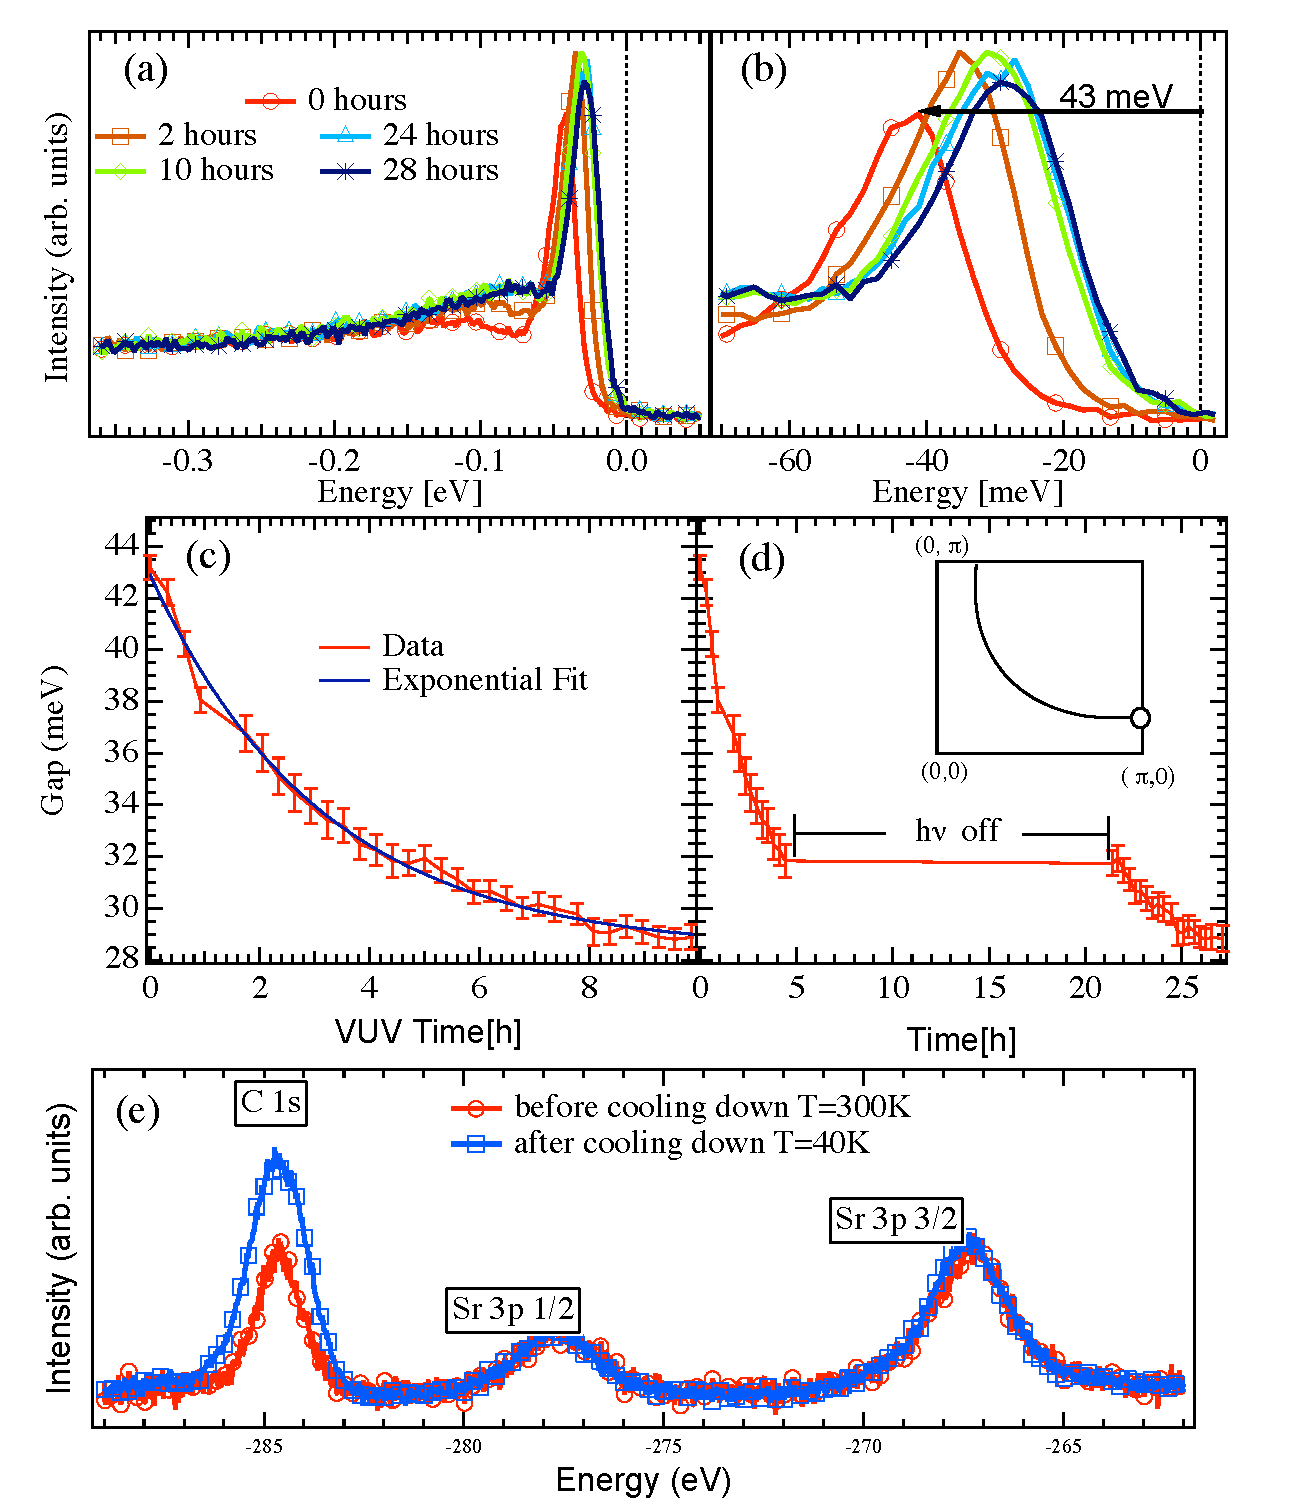
\includegraphics[width=3.6in]{fig1.pdf}
\caption{Color online) ARPES specta of Bi2212 taken under poor vacuum
conditions (a) sample EDC (energy distribution curves) taken at the
anti-node where the band crosses the Fermi energy at 5 different
times, (b) narrow view of (a), (c) time evolution of Bi2212's
superconducting gap as a function of tine, (d) the time evolution of
Bi2212's superconducting gap under VUV photons (red) fitted with an
exponential decay (blue), the temperature for (a)-(d) was set to 20K, 
(e) C 1s, Sr 3P 1/2, Sr 3p 3/2 core level data from Bi2212 showing
carbon deposits some time after cleaving and after while cooling.}
\label{Fig. 1}
\end{figure}
%%%%%%%%%%%%%%%%%%%%%%

%%%%%%%%%%%%%%%%%%%%% bilayer splitting
\begin{figure}
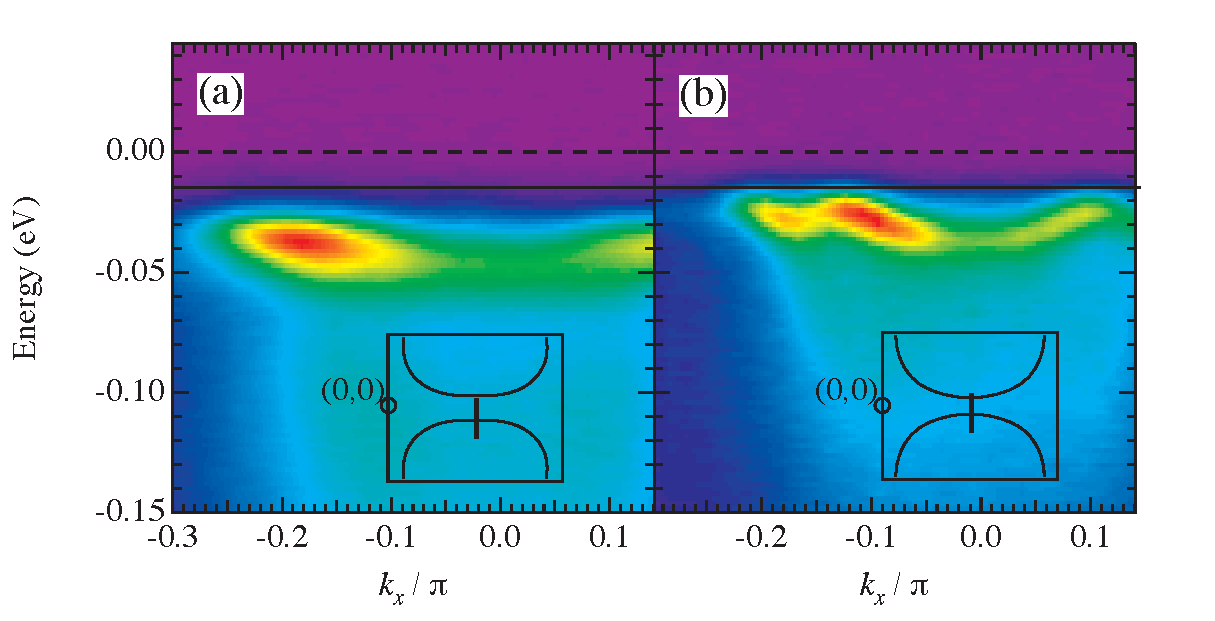
\includegraphics[width=3.6in]{fig2.pdf}
\caption{(Color online) (a) ARPES intensity map of freshly cleaved
optimally doped Bi2212 at ($\pi$, 0) showing no bilayer splitting, (b)
ARPES intensity maps on the same sample and the same location as in
(a) only oxygen aged (\textit{in-situ} overdoing) in a UHV system with
a leak showing bilayer splitting and a peak shift location of the
Fermi momentum, with the black line as a guide to the eye.}
\label{Fig. 2}
\end{figure}
%%%%%%%%%%%%%%%%%%%%%%

n absence of leaks, a reasonable UHV system has normally undetectable
levels of oxygen. However in stainless steel vessels CO and CO$_2$ are
always present. These oxide molecules can adhere to clean sample
surfaces especially at low temperatures. When the molecules are
exposed to VUV photons above 6 eV they break into carbon and oxygen
\cite{M. M. Halmann}; the oxygen can then be incorporated into BiO
layer as dopant, while the carbon atoms remain on the surface. The
proof of this scenario is in Fig. 1 (e) where the core-level spectrum
of Bi2212 at 300K and 40K are shown.  As the sample cooled more CO and
CO$_2$ molecules adhered to the surface of the sample. Since there are
carbon deposits some time after cleaving and even more after cooling,
it is likely the oxygen accompanied the carbon to the surface.  This
oxygen can then change the doping of the sample after it is
dissociated from the carbon. 

%%%%%%%%%%%%%%%%%%%%% before and after heating up with 280K time
evolution spectrum
\begin{figure}
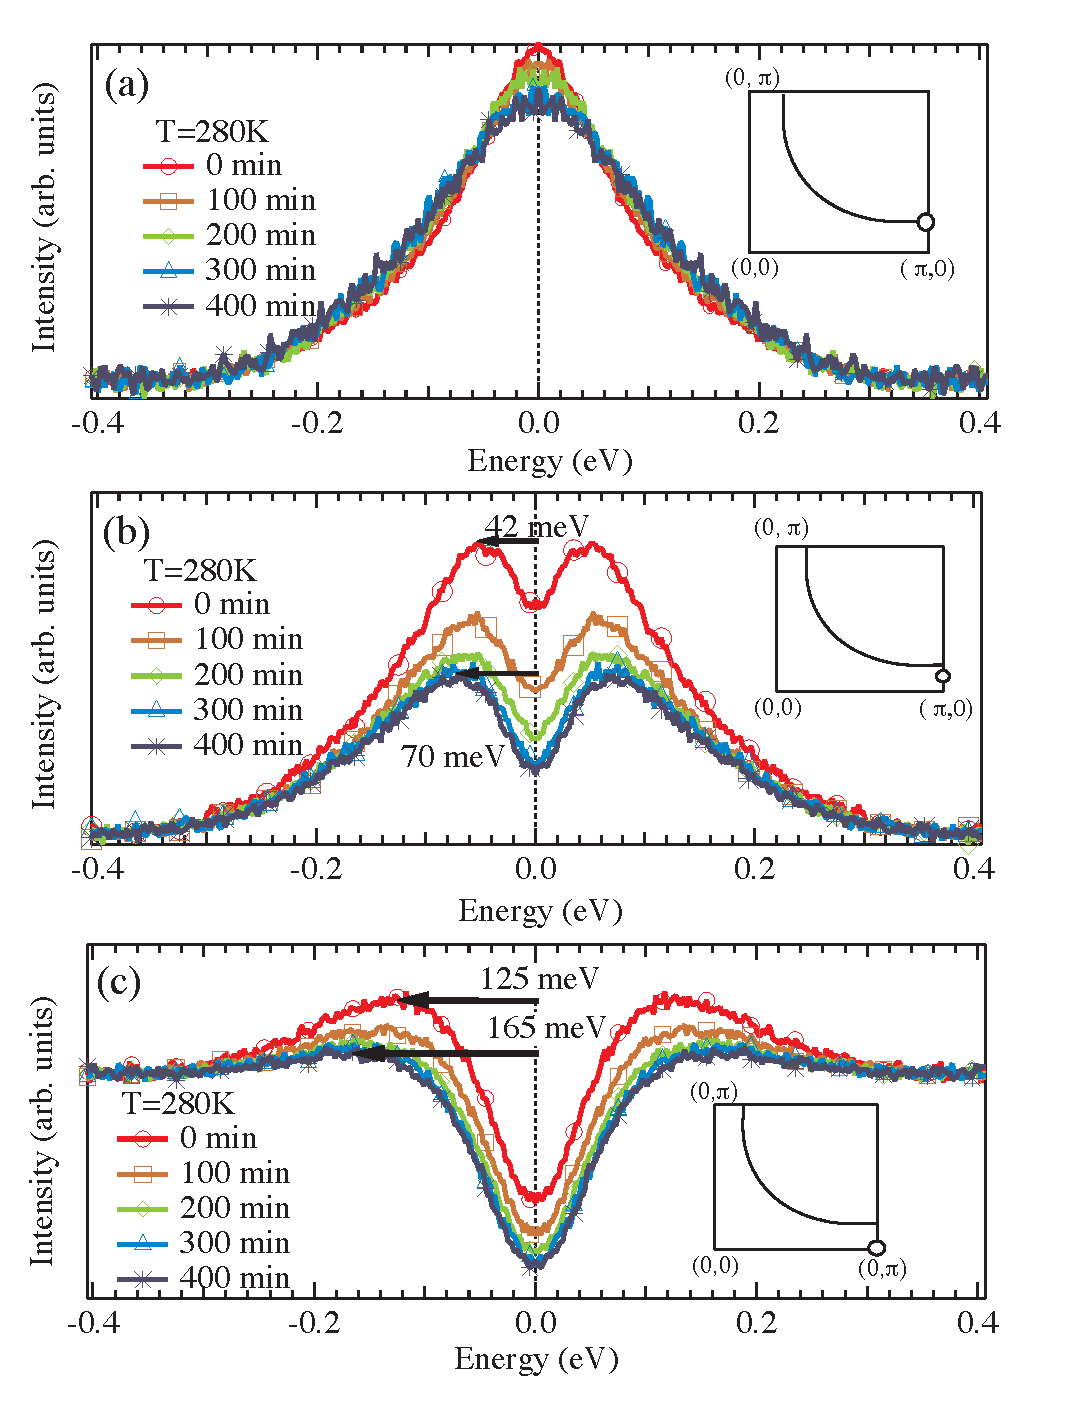
\includegraphics[width=3.2in]{fig3.pdf}
\caption{(Color online) (a)-(c) symmetrized ARPES EDC's for Bi2212
taken at three points near ($\pi$,0) showing the time evolution of the
spectrum at 280K.}
\label{Fig. 2}
\end{figure}
%%%%%%%%%%%%%%%%%%%%%%

In the presence of a leak a UHV system can have detectable amounts of
oxygen.  Under these conditions a Bi2212 sample can age even without
the breakdown of CO and CO$_2$.  One of the trademarks of an
over-doped (aged) Bi2212 sample is the appearance of bi-layer band
splitting at the antinode ($\pi$, 0).  While there has been a
relatively active discussion on whether Bi2212 contains bilayer band
splitting all the time or just in an over-doped state; bilayer
splitting has only been seen in over-doped samples when using a helium
discharge lamp \cite{Y.-D. Chaung 2004, S. V. Borisenko 2004, S. V.
Borisenko 2006, A. A. Kordyuk 2004}. An example of this is shown in
FIG. 2 where a fresh Bi2212 sample was scanned and then allowed to sit
in the leaky UHV system overnight before scanning again. Even though
the sample was kept a 20 K, bilayer band splitting was detected after
the break, signaling that the sample aged because of oxygen
absorption.

\section{Decreasing carrier concentration}
%%%%%%%%%%%%%%%%%%%%%gap plots before and after heating up
\begin{figure}
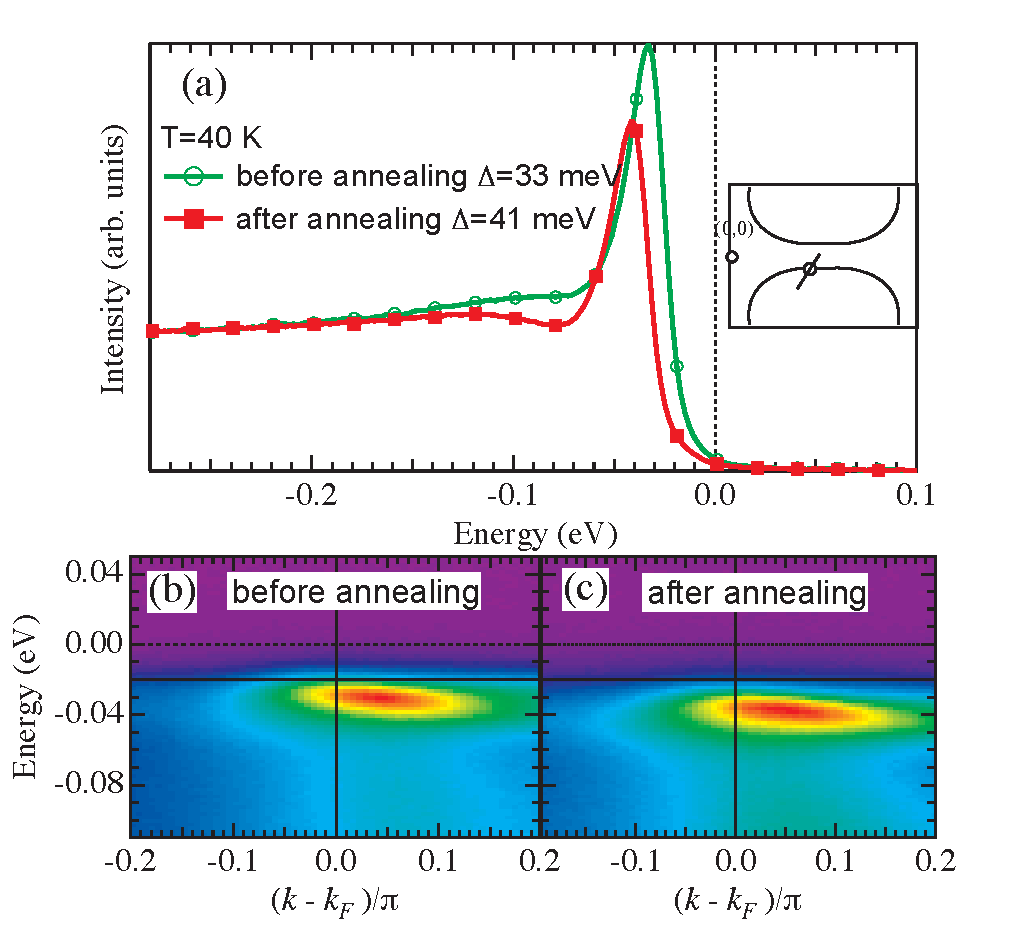
\includegraphics[width=3.6in]{fig4.pdf}
\caption{(Color online) (a) EDC at the Fermi momentum close to the
anti-node before (green circles) and after (solid red squares)
annealing at 280K over 28 hours with their respective superconducting
gaps $\Delta$, (b)-(c) momentum intensities maps taken across Fermi
momentum close to ($\pi$, 0) before and after annealing.}
\label{Fig. 3}
\end{figure}
%%%%%%%%%%%%%%%%%%%%%%


While in a reasonable vacuum system there can be enough CO$_2$/CO to
change the surface doping of a sample over time; in an ultra clean UHV
system samples can live for many weeks without surface degradation or
a change in doping (assuming the sample is kept at low temperature). 
Yet, when the sample is annealed above 200K an interesting thing
happens to the Bi2212's doping level; the sample doping level is
reduced (the opposite of aging).  This is seen in Fig. 3 (a)-(c) where
the time evolution of Bi2212's EDCs at three locations at or near
($\pi$,0) with the sample at 280K is shown.  The sample actually
changes doping moving towards lower doping (signified by a larger
spectral gap). Fig. 4 (a) shows the energy distribution curve (EDC) at
the anti-nodal Fermi momentum from the same sample before and after
annealing at 280K for 28 hours.  The superconducting gap clearly
shifts from 33 meV to 41 meV and the peak is suppressed, signaling
that the doping has changed from a slightly over doped sample to a
more under doped sample\cite{T. Sato 2001}.   The momentum color maps
from Fig. 4 (a) are shown in FIG. 4 (b)-(c); after annealing the gap
shifts to higher binding energy, there is also a shift in the location
of the Fermi momentum.  This momentum shift comes from a change in the
chemical potential, which moves lower in a ridged-band-like fashion
upon doping.\cite{M. Hashimoto 2008}






Another way to see if a samples carrier concentration has decreased is
to look at the pseudogap.  Fig. 5 (a) shows the EDC at the Fermi
momentum before and after annealing at 280K for 28 hours.  The
pseudogap shifts from 30 meV to 50 meV.  As Bi2212 goes to lower
doping levels the pseudogap becomes bigger and the temperature at
which the pseudogap remains (T*) becomes higher\cite{H. Ding 1996}.
Fig. 5 (b)-(c) demonstrates that before annealing T* is below 140K
with the pseudogap disappearing and after annealing T* is above 200K. 
The pseudogap after annealing is above 200K, which guarantees that the
sample is at a lower doping level.

%%%%%%%%%%%%%%%%%%%%%gap while annealing
\begin{figure}
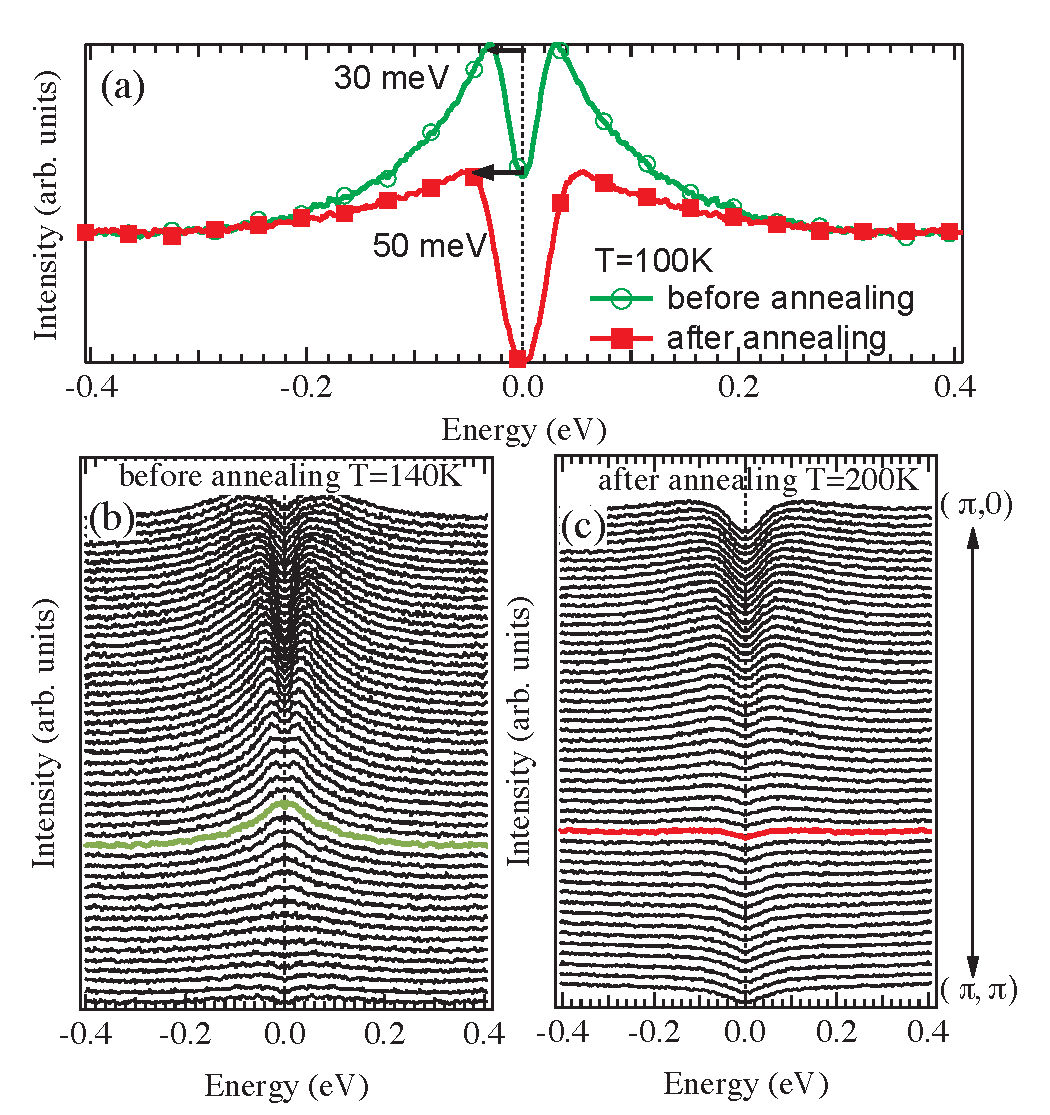
\includegraphics[width=3.6in]{fig5.pdf}
\caption{(Color online)  (a) 100 K symmetrized ARPES data taken at the
Fermi momentum before and after annealing at 280 K for 28 hours, (b)
ARPES intensities at 140 K before annealing, (c) ARPES intensities at
200 K after annealing.}
\label{Fig. 4}
\end{figure}
%%%%%%%%%%%%%%%%%%%%%%



Until now we have only shown the lowering of doping on Bi2212 at
elevated temperature.  While we still haven't shown if the doping
change is caused by the elevated temperature or a combination of
elevated temperature and VUV photons.  This was tested by scanning the
sample just after cleaving and again after the sample sat under UHV
for 16 days at 100K. This data is shown in figure Fig. 6 (a).  The
spectrum barely changed over the two weeks. While in Fig. 6 (b) we
show the 280K spectrum just after cleaving, and again after the sample
sat under UHV for 8 days at 280K.  Most of the spectral weight has
shifted to higher energies and the Fermi edge has all but disappeared,
signifying an almost completely insulating sample. From Fig. 6 we can
conclude that the lowering of the samples doping is only caused by the
elevated temperatures.

%%%%%%%%%%%%%%%%%%%%%doping over a week
\begin{figure}
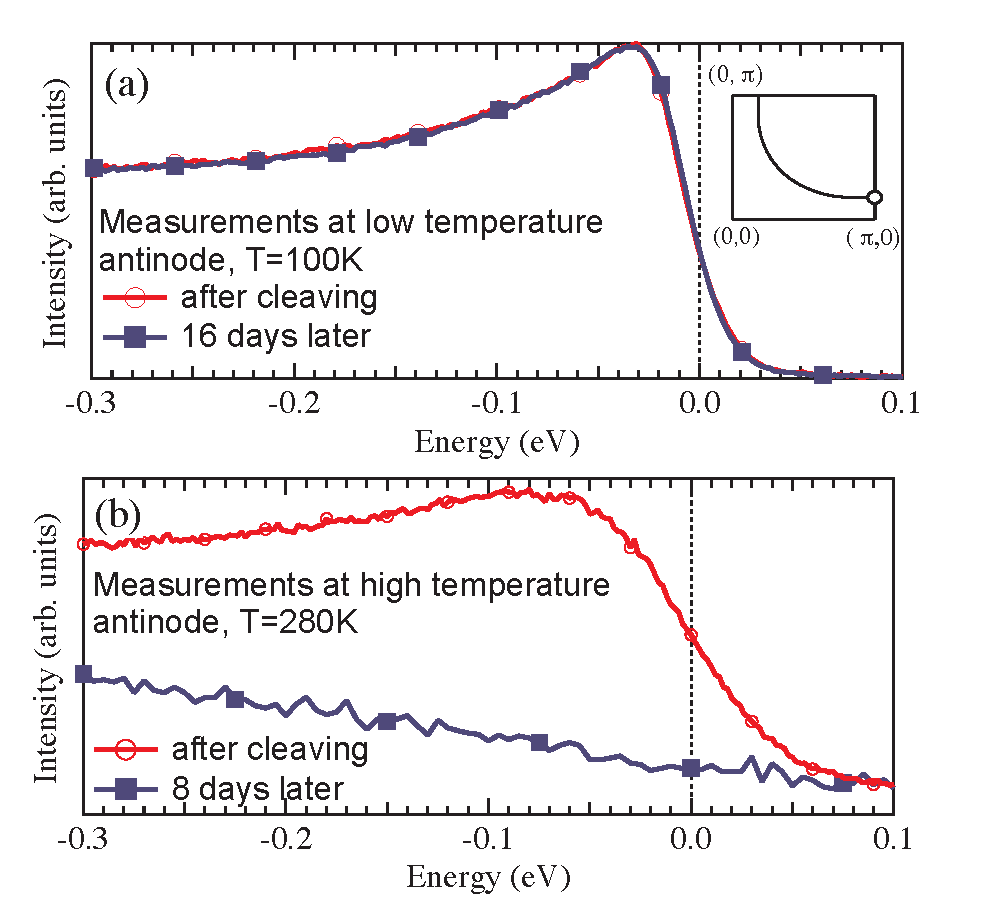
\includegraphics[width=3.6in]{fig6.pdf}
\caption{(Color online) Bi2212 EDC at the Fermi momentum close to
($\pi$,0) (a) just after cleaving at 100K (red circles) and again
after sitting at 100K for 16 days (solid blue squares), (b) just after
cleaving at 280K (red circles) and again after sitting at 280K for 8
days (solid blue squares).}
\label{Fig. 5}
\end{figure}
%%%%%%%%%%%%%%%%%%%%%%


%%%%%%%%%%%%%%%%%%%%%proof of principle
\begin{figure*}
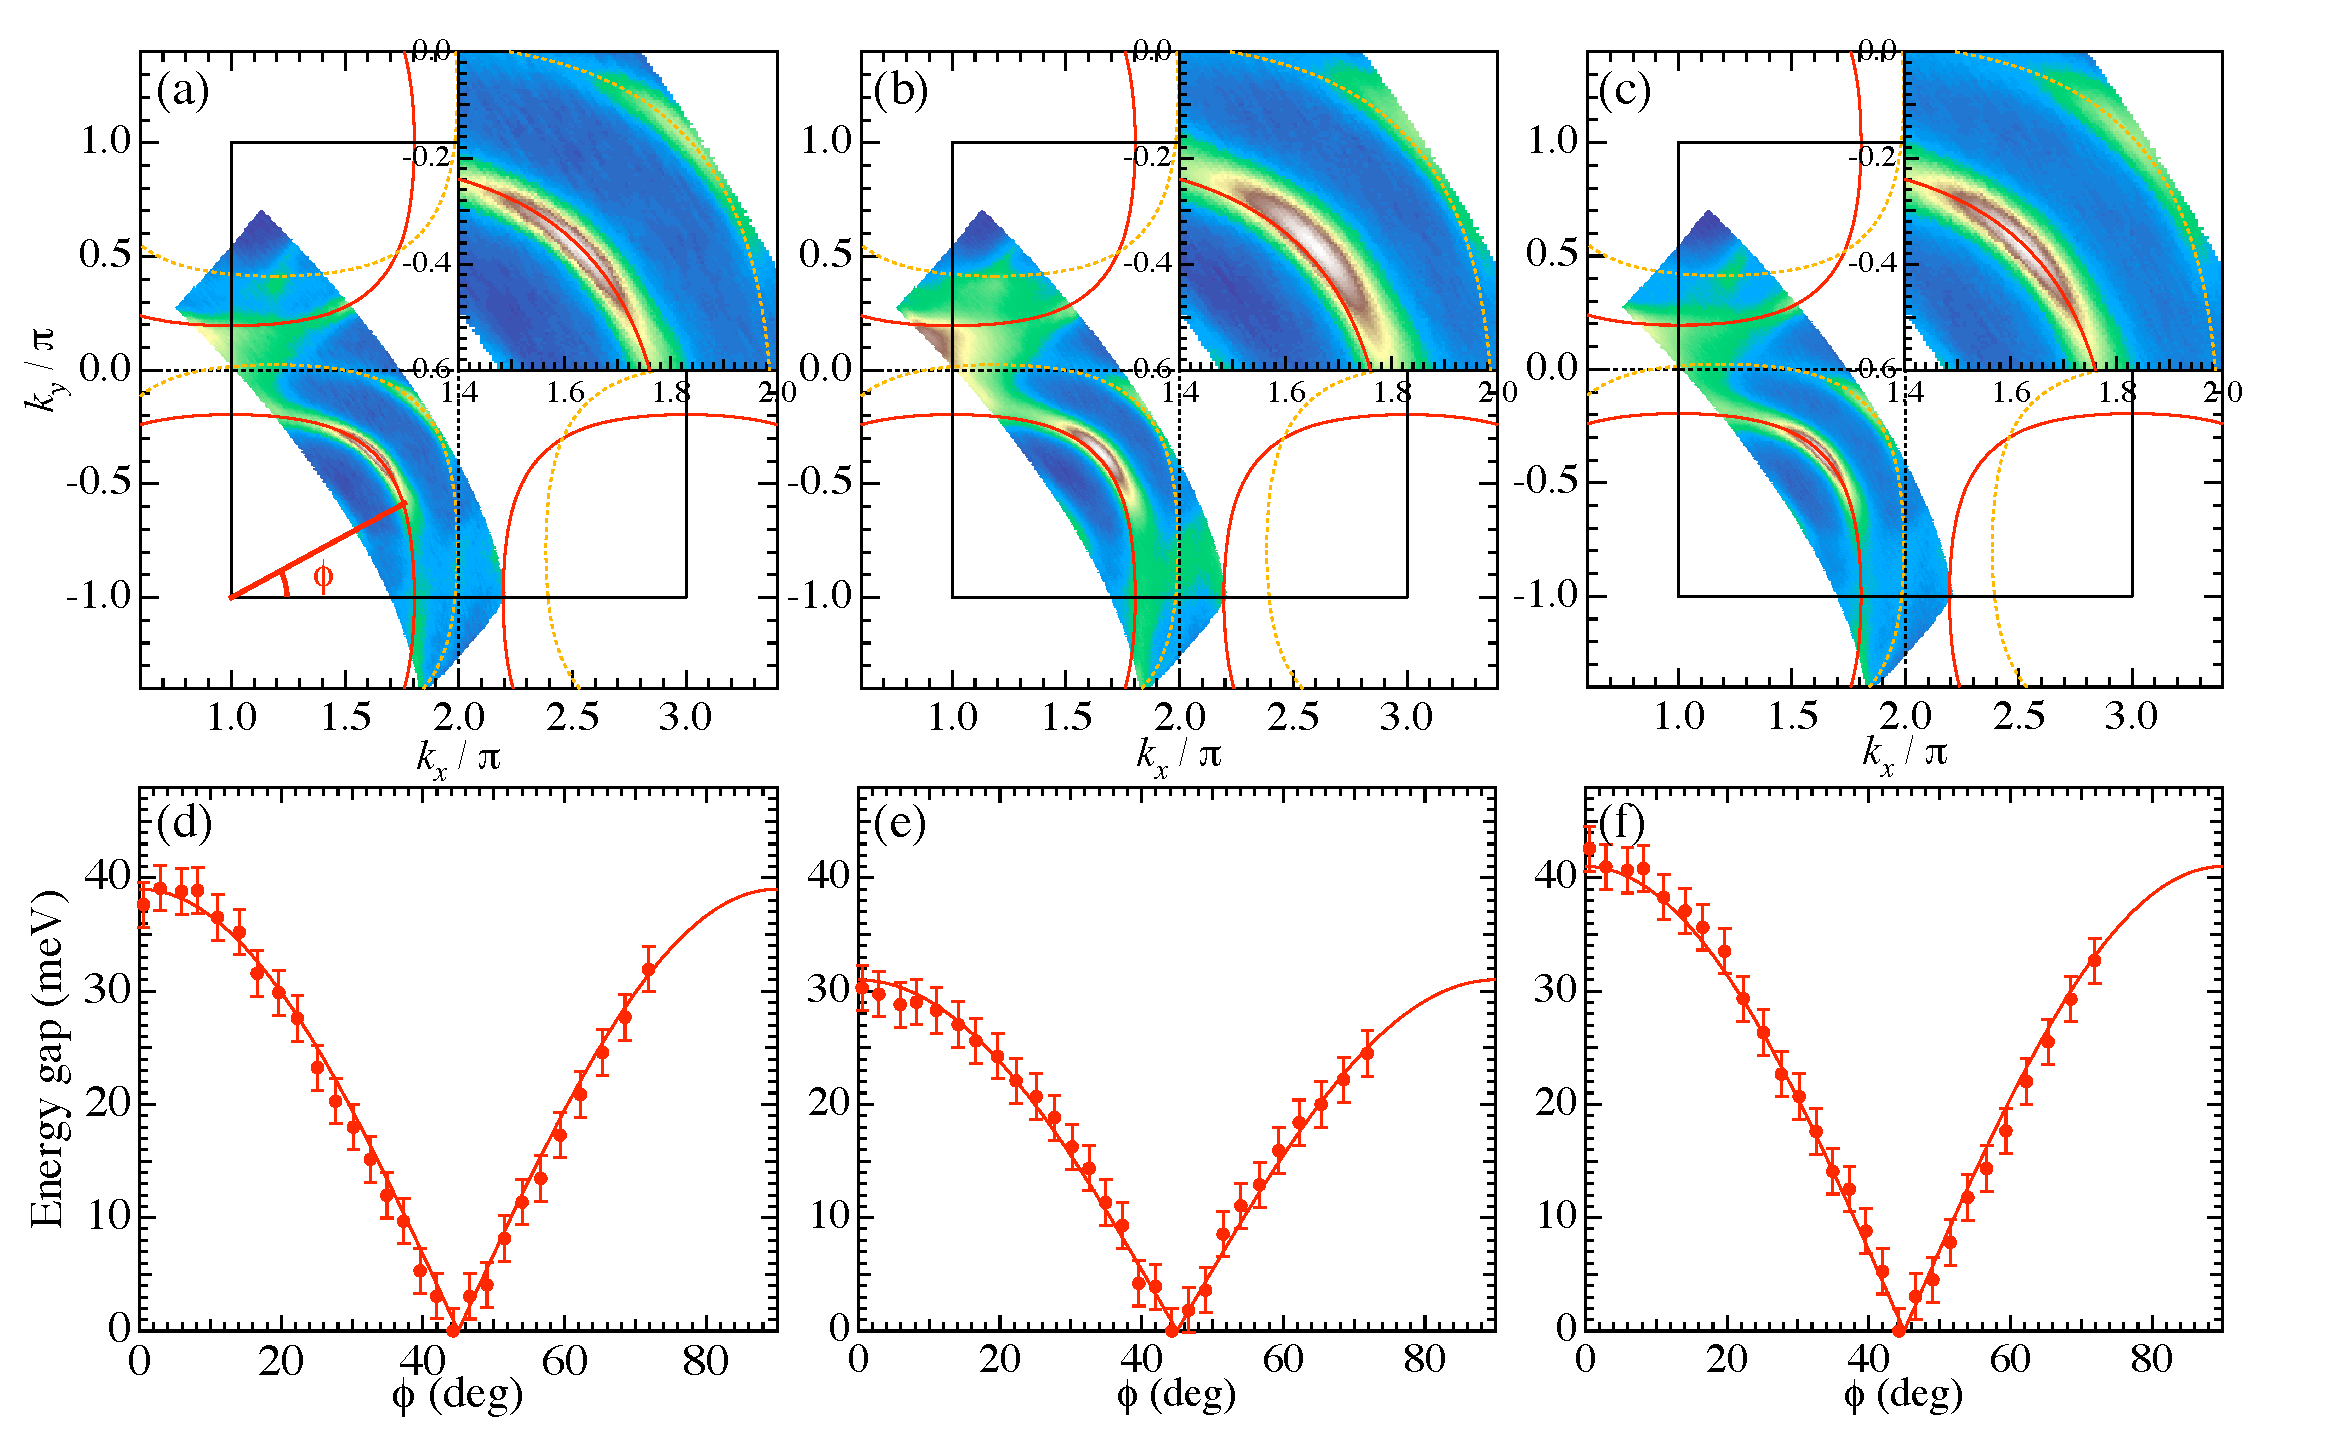
\includegraphics[width=6 in]{fig7.pdf}
\caption{(Color online) ARPES intensity plots at the Fermi energy from
the same sample at three different times all at 12K: (a) just after
cleaving, (b) after a couple of days of VUV aging at low temperature,
(c) after annealing at 280K overnight; the upper right hand corner of
(a)-(c) are the zoomed in images from the bottom left hand corner, the
red and dotted yellow curves are from a tight binding fit for
optimally doped Bi2212 as a guide to the eye, (d)-(f) the size of the
superconducting gap as a function of angle $\phi$ from (a)-(c)
respectively.}
\label{Fig. 6}
\end{figure*}
%%%%%%%%%%%%%%%%%%%%%%

The greatest consequence of this study is that Bi2212's doping can be
change from over doped all the way down to insulating in a systematic
fashion on a single crystal. To this point the data presented has been
either over doped by aging or under doped by annealing on different
samples.  Fig. 7 demonstrates how a \textit{single} sample can be
over-doped by aging and then under-doped by annealing to move across
the phase diagram. An optimally doped Bi2212 sample was cleaved, the
Fermi surface and superconducting gap values as a function of angle
$\phi$ (angle clockwise from the line ($\pi$,-$\pi$) to (2
$\pi$,-$\pi$)) was scanned Fig. 7 (a) $\&$ (d).  Aging was detected
after a couple of days of scanning Fig. 7 (b) $\&$ (e).  The sample
was then annealed overnight at 280K to remove the aging Fig. 7 (c)
$\&$ (f).

\section{Conclusion}

We have presented a systematic study of the electronic properties at
the surface of Bi2212 as a function of vacuum conditions.  The results
confirm that under poor vacuum conditions there is an increase in
carrier concentration due to the breakup of CO and CO$_2$ molecules by
exposure to vacuum ultra-violet (VUV) photons and a subsequent
adsorption of oxygen into the BiO layers. We also show that with a UHV
leak a sample can increase its carrier concentration just by sitting
in the vaccum.  This observation confirms that bilayer splitting only
occurs in over-doped Bi2212. We then show that at elevated
temperatures (T$>$200K) the sample surface loses oxygen, which results
in a reduction of the carrier concentration.  These two effects
(\textit{in-situ} absorption and desorption of oxygen) can be utilized
in order to control the carrier concentration of Bi2212. This approach
enables one to study the intrinsic electronic properties (i.e. without
changing the impurities and defects) of the cuprates across the phase
diagram in ARPES as well as other surface sensitive techniques on a
single sample.

\section{Acknowledgments}

This work was supported by Director Office for Basic Energy Sciences,
US DOE. Work at Ames Laboratory was supported by the Department of
Energy - Basic Energy Sciences under Contract No. DE-AC02-07CH11358. 
The work at BNL was supported by Department of Energy - Basic Energy
Sciences under Contract No. DE-AC02-98CH10886. Synchrotron Radiation
Center is supported by the National Science Foundation under award No.
DMR-0537588.

\begin{thebibliography}{99}

\bibitem{OLSON}
C. G. Olson, R. Liu, A. -B. Yang, D. W. Lynch, A. J. Arko, R. S. List,
B. W. Veal, Y. C. Chang, P. Z. Jiang, A. P. Paulikas. Science {\bf
245}, 731 (1989).

\bibitem{SHENSC}
Z.-X. Shen, D.S. Dessau, B.O. Wells, D.M. King, W.E. Spicer, A.J.
Arko, D.S. Marshall, L.W. Lombardo, A. Kapitulnik, P. Dickinson, S.
Doniach, J. Dicarlo, T. Loeser, C.H. Park Phys. Rev. Lett. {\bf70},
1553 (1993).

\bibitem{HONGSC}
H. Ding, M. R. Norman, J. C. Campuzano, M. Randeria, A. F. Bellman, T.
Yokoya, T. Takahashi, T. Mochiku, K. Kadowaki, Phys, Rev, B, {\bf54},
R9678 (1996).

\bibitem{HONGPG}
H. Ding, T. Yokoya, J. C. Campuzano, T. Takahashi, M. Randeria, M. R.
Norman, T. Mochiku, K. Kadowaki, J. Giapintzakis, Nature {\bf382}, 51
(1996).

\bibitem{LOESERPG} Loeser, A.G. {\it et al.} Excitation gap in the
normal state of underdoped Bi$_{2}$$Sr_{2}$CaCu$_{2}$O$_{8+\delta}$.
{\it Science} {\bf 273}, 325-329 (1996).

\bibitem{MIKEPG}
M. R. Norman, H. Ding, M. Randeria, J. C. Campuzano, T. Yokoya, T.
Takeuchi, T. Takahashi, T. Mochiku, K. Kadowaki, P. Guptasarma, D. G.
Hinks, Nature {\bf392}, 157 (1998).

\bibitem{DAVIS}
S. H. Pan J. P. O'Neal R. L. Badzey C. Chamon H. Ding J. R.
Engelbrecht Z. Wang H. Eisaki S. Uchida A. K. Gupta K.-W. Ng E. W.
Hudson K. M. Lang, J. C. Davis, Nature {\bf 413}, 282 (2001).

\bibitem{YAZDANI}
K. K. Gomes, A. N. Pasupathy, A. Pushp, S. Ono, Y. Ando, A. Yazdani,
Nature (London) {\bf447}, 569 (2007).

\bibitem{DAVISCHECKER}
T. Hanaguri, C. Lupien, Y. Kohsaka, D. -H. Lee, M. Azuma, M. Takano,
H. Takagi and J. C. Davis, Nature {\bf430}, 1001 (2004).

\bibitem{KAMINSKIQP}
A. Kaminski, J. Mesot, H. Fretwell, J. C. Campuzano, M. R. Norman, M.
Randeria, H. Ding, T. Sato, T. Takahashi, T. Mochiku, K. Kadowaki, H.
Hoechst, Phys. Rev. Lett. {\bf84}, 1788 (2000).

\bibitem{VALLA}
T. Valla, T. E. Kidd, W.-G. Yin, G. D. Gu, P. D. Johnson, Z.-H. Pan,
A. V. Fedorov, Phys. Rev. Lett. {\bf98}, 167003 (2007).

\bibitem{BOGDANOV}
P. V. Bogdanov, A. Lanzara, S. A. Kellar, X. J. Zhou, E. D. Lu, W. J.
Zheng, G. Gu, J.-I. Shimoyama, K. Kishio, H. Ikeda, R. Yoshizaki, Z.
Hussain, Z. X. Shen, Phys. Rev. Lett. {\bf85}, 2581 (2000).

\bibitem{KAMINSKIKINK}
A. Kaminski, M. Randeria, J. C. Campuzano, M. R. Norman, H. Fretwell,
J. Mesot, T. Sato, T. Takahashi, K. Kadowaki, Phys. Rev. Lett.
{\bf86}, 1070 (2001).

\bibitem{SHENREVIEW}
A. Damascelli, Z. Hussain and Z.-X. Shen, Rev. Mod. Phys. {\bf75}, 473
(2003).

\bibitem{JCREVIEW}
J. C. Campuzano, M. R. Norman, M. Randeria, in {\it The Physics of
Superconductors}, Vol. 2, ed. K. H. Bennemann and J. B. Ketterson
(Springer, Berlin, 2004), p. 167.

\bibitem{SHEN1}
Z.-X. Shen, D. S. Dessau, B. O. Wells, D. M. King, W. E. Spicer, A. J.
Arko, D. Marshall, L. W. Lombardo, A. Kapitulnik, P. Dickinson, S.
Doniach, J. DiCarlo, T. Loeser, C. H. Park, Phys. Rev. Lett. {\bf70},
1553 (1993).

\bibitem{A. A. Kordyuk 2008}
A. A. Kordyuk, S. V. Borisenko, V. B. Zabolotnyy, R. Schuster, D. S.
Inosov, R. Follath, A. Varykhalov, L. Patthey, H. Berger
arXiv:0801.2546 (2008).

\bibitem{H. Ding 1997}
H. Ding, M. R. Norman, T. Yokoya, T. Takeuchi, M. Randeria, J. C.
Campuzano, T. Takahashi, T. Mochiku, K. Kadowaki, Phys. Rev. Lett.
{\bf78}, 2628 (1997).

\bibitem{P. Schwaller 2000}
P. Schwaller, T. Greber, P. Aebi, J.M. Singer, H. Berger, L. Forr� and
J. Osterwalder, Eur Phys. J. B {\bf18}, 215 (2000).

\bibitem{M. M. Halmann}
M. M. Halmann, M. Steinberg, Greenhouse Gas Carbon Dioxide Migration,
p. 47,  CRC press (1998).

\bibitem{Y.-D. Chaung 2004}
Y.-D. Chuang, A. D. Gromko, A. V. Fedorov, Y. Aiura, K. Oka, Yoichi
Ando, M. Lindroos, R. S. Markiewicz, A. Bansil, D. S. Dessau, Phys.
Rev. B {\bf69}, 094515 (2004)

\bibitem{S. V. Borisenko 2004}
S. V. Borisenko, A. A. Kordyuk, S. Legner, T. K. Kim, M. Knupfer, C.
M. Schneider, J. Fink, M. S. Golden, M. Sing, R. Claessen, A. Yaresko,
H. Berger, C. Grazioli, S. Turchini Phys. Rev. B {\bf69}, 224509
(2004)

\bibitem{S. V. Borisenko 2006}
S. V. Borisenko, A. A. Kordyuk, A. Koitzsch, J. Fink, J. Geck, V.
Zabolotnyy, M. Knupfer, B. B�chner, H. Berger, M. Falub, M. Shi, J.
Krempasky, L. Patthey, Phys. Rev. Lett. {\bf96}, 067001 (2006)

\bibitem{A. A. Kordyuk 2004}
A. A. Kordyuk, S. V. Borisenko, A. N. Yaresko, S.-L. Drechsler, H.
Rosner, T. K. Kim, A. Koitzsch, K. A. Nenkov, M. Knupfer, J. Fink, R.
Follath, H. Berger, B. Keimer, S. Ono, Yoichi Ando, Phys. Rev. B
{\bf70}, 214525 (2004)

\bibitem{T. Sato 2001}
T. Sato, T. Kamiyama, Y. Naitoh, T. Takahashi, I. Chong, T. Terashima,
M. Takano, Phys. Rev. B {\bf63}, 132502 (2001).

\bibitem{M. Hashimoto 2008}
M. Hashimoto, T. Yoshida, H. Yagi, M. Takizawa, A. Fujimori, M.
Kubota, K. Ono, K. Tanaka, D.H. Lu, Z.-X. Shen, S. Ono, Yoichi Ando,
arXiv:0801.0782v2 (2008)

\bibitem{H. Ding 1996}
H. Ding, T. Yokoya, J. C. Campuzano, T. Takahashi, M. Randeria, M. R.
Norman, T. Mochikuparallel, K. Kadowakiparallel J. Giapintzakis,
Nature {\bf382}, 51 (1996).


\end{thebibliography}

\end{document}

